%% bare_conf.tex
%% V1.4b
%% 2015/08/26
%% by Michael Shell
%% See:
%% http://www.michaelshell.org/
%% for current contact information.
%%
%% This is a skeleton file demonstrating the use of IEEEtran.cls
%% (requires IEEEtran.cls version 1.8b or later) with an IEEE
%% conference paper.
%%
%% Support sites:
%% http://www.michaelshell.org/tex/ieeetran/
%% http://www.ctan.org/pkg/ieeetran
%% and
%% http://www.ieee.org/

%%*************************************************************************
%% Legal Notice:
%% This code is offered as-is without any warranty either expressed or
%% implied; without even the implied warranty of MERCHANTABILITY or
%% FITNESS FOR A PARTICULAR PURPOSE! 
%% User assumes all risk.
%% In no event shall the IEEE or any contributor to this code be liable for
%% any damages or losses, including, but not limited to, incidental,
%% consequential, or any other damages, resulting from the use or misuse
%% of any information contained here.
%%
%% All comments are the opinions of their respective authors and are not
%% necessarily endorsed by the IEEE.
%%
%% This work is distributed under the LaTeX Project Public License (LPPL)
%% ( http://www.latex-project.org/ ) version 1.3, and may be freely used,
%% distributed and modified. A copy of the LPPL, version 1.3, is included
%% in the base LaTeX documentation of all distributions of LaTeX released
%% 2003/12/01 or later.
%% Retain all contribution notices and credits.
%% ** Modified files should be clearly indicated as such, including  **
%% ** renaming them and changing author support contact information. **
%%*************************************************************************

% *** Authors should verify (and, if needed, correct) their LaTeX system  ***
% *** with the testflow diagnostic prior to trusting their LaTeX platform ***
% *** with production work. The IEEE's font choices and paper sizes can   ***
% *** trigger bugs that do not appear when using other class files.       ***
% The testflow support page is at:
% http://www.michaelshell.org/tex/testflow/

\documentclass[12pt,twoside,a4paper,openright]{report}
\usepackage{etex}
% Select encoding of your inputs.
\usepackage[utf8]{inputenc}

% Make latex understand and use the typographic
% rules of the language used in the document.
\usepackage[english, danish]{babel}

% Use the vector font Latin Modern which is going
% to be the default font in latex in the future.
\usepackage{lmodern}

% Choose the font encoding
\usepackage[T1]{fontenc}

% Use colour in tables
\usepackage[table]{xcolor}
\usepackage{array}
\usepackage{multirow}

% load a colour package
\usepackage{xcolor}
\definecolor{aaublue}{RGB}{33,26,82}% dark blue

% The standard graphics inclusion package
\definecolor{white}{RGB}{255,255,255} % define color white
\usepackage{graphicx}
\usepackage{adjustbox}

% Set up how figure and table captions are displayed
\usepackage{caption}
\captionsetup{
  font=footnotesize,% set font size to footnotesize
  labelfont=bf % bold label (e.g., Figure 3.2) font
}

% Enable row combination in tables
\usepackage{multirow}

% Make space between table lines and text
\renewcommand{\arraystretch}{1.5}

% Make the standard latex tables look so much better
\usepackage{array,booktabs}

% Enable the use of frames around, e.g., theorems
% The framed package is used in the example environment
\usepackage{framed}
\usepackage{colortbl}
\usepackage{longtable}
\usepackage{xcolor}
\usepackage{textcomp}

%%%%%%%%%%%%%%%%%%%%%%%%%%%%%%%%%%%%%%%%%%%%%%%%
% Mathematics
%%%%%%%%%%%%%%%%%%%%%%%%%%%%%%%%%%%%%%%%%%%%%%%%
% Defines new environments such as equation,
% align and split 
\usepackage{amsmath}
\usepackage{relsize}
% Adds new math symbols
\usepackage{amssymb}
% Use theorems in your document
% The ntheorem package is also used for the example environment
% When using thmmarks, amsmath must be an option as well. Otherwise \eqref doesn't work anymore.
\usepackage[framed,amsmath,thmmarks]{ntheorem}
\usepackage{cancel}

%%%%%%%%%%%%%%%%%%%%%%%%%%%%%%%%%%%%%%%%%%%%%%%%
% Page Layout
%%%%%%%%%%%%%%%%%%%%%%%%%%%%%%%%%%%%%%%%%%%%%%%%
% Change margins, papersize, etc of the document
\usepackage[
  left=25mm,% left margin on an odd page %tidligere 25mm for baade right og left
  right=25mm,% right margin on an odd page
  top=35mm,
  ]{geometry}
  
% Modify how \chapter, \section, etc. look
% The titlesec package is very configureable
\usepackage{titlesec}
\makeatletter
\def\ttl@mkchap@i#1#2#3#4#5#6#7{%
    \ttl@assign\@tempskipa#3\relax\beforetitleunit
    \vspace{\@tempskipa}%<<<<<< REMOVE THE * AFTER \vspace
    \global\@afterindenttrue
    \ifcase#5 \global\@afterindentfalse\fi
    \ttl@assign\@tempskipb#4\relax\aftertitleunit
    \ttl@topmode{\@tempskipb}{%
        \ttl@select{#6}{#1}{#2}{#7}}%
    \ttl@finmarks  % Outside the box!
    \@ifundefined{ttlp@#6}{}{\ttlp@write{#6}}}
\makeatother

\titlespacing{\chapter}{0pt}{0pt}{10pt}
\titlespacing{\section}{0pt}{0pt}{-5pt}
\titlespacing{\subsection}{0pt}{8pt}{-5pt}
\titlespacing{\subsubsection}{0pt}{6pt}{-10pt}

\titleformat*{\section}{\normalfont\Large\bfseries\color{aaublue}}
\titleformat*{\subsection}{\normalfont\large\bfseries\color{aaublue}}
\titleformat*{\subsubsection}{\normalfont\normalsize\bfseries\color{aaublue}}

\usepackage{bookmark}
\usepackage{titlesec, blindtext, color}
%\color{gray75}{gray}{0.75}
\newcommand{\hsp}{\hspace{20pt}}
\titleformat{\chapter}[hang]{\Huge\bfseries}{\thechapter\hsp\textcolor{aaublue}{|}\hsp}{0pt}{\Huge\bfseries}

% Change the headers and footers
\usepackage{fancyhdr}
\setlength{\headheight}{15pt}
\pagestyle{fancy}
\fancyhf{} %delete everything
\renewcommand{\headrulewidth}{0pt} %remove the horizontal line in the header
\fancyhead[RO,LE]{\color{aaublue}\small\nouppercase\leftmark} %even page - chapter title
\fancyhead[LO]{}
\fancyhead[RE]{} 
\fancyhead[CE]{}
\fancyhead[CO]{}
\fancyfoot[RE,LO]{\thepage}
\fancyfoot[LE,RO]{} %page number on all pages
\fancyfoot[CE,CO]{}

% change first page of all chapters header and footer to fancy style
\makeatletter
\let\ps@plain\ps@fancy
\makeatother

% Do not stretch the content of a page. Instead,
% insert white space at the bottom of the page
\raggedbottom

% Enable arithmetics with length. Useful when typesetting the layout.
\usepackage{calc}

%%%%%%%%%%%%%%%%%%%%%%%%%%%%%%%%%%%%%%%%%%%%%%%%
% Bibliography
%%%%%%%%%%%%%%%%%%%%%%%%%%%%%%%%%%%%%%%%%%%%%%%%
%setting references (using numbers) and supporting i.a. Chicargo-style:
\usepackage{etex}
\usepackage{etoolbox}
\usepackage{keyval}
\usepackage{ifthen}
\usepackage{url}
\usepackage{csquotes}
\usepackage[backend=biber, url=true, doi=true, style=numeric, sorting=none]{biblatex}
\addbibresource{setup/bibliography.bib}

%%%%%%%%%%%%%%%%%%%%%%%%%%%%%%%%%%%%%%%%%%%%%%%%
% Misc
%%%%%%%%%%%%%%%%%%%%%%%%%%%%%%%%%%%%%%%%%%%%%%%%

%%% Enables the use FiXme refferences. Syntax: \fxnote{...} %%%
\usepackage[footnote, draft, english, silent, nomargin]{fixme}
%With "final" instead of "draft" an error will ocure for every FiXme under compilation.

%%% allows use of lorem ipsum (generate i.e. pagagraph 1 to 5 with \lipsum[1-5]) %%%
\usepackage{lipsum}

%%% Enables figures with text wrapped tightly around it %%%
\usepackage{wrapfig}

%%% Section debth included in table of contents (1 = down to sections) %%%
\setcounter{tocdepth}{1}

%%% Section debth for numbers (1 = down to sections) %%%
\setcounter{secnumdepth}{1}

\usepackage{tocloft}
\setlength{\cftbeforetoctitleskip}{0 cm}
\renewcommand{\cftpartpresnum}{Part~}
\let\cftoldpartfont\cftpartfont
\renewcommand{\cftpartfont}{\cftoldpartfont\cftpartpresnum}

%%%%%%%%%%%%%%%%%%%%%%%%%%%%%%%%%%%%%%%%%%%%%%%%
% Hyperlinks
%%%%%%%%%%%%%%%%%%%%%%%%%%%%%%%%%%%%%%%%%%%%%%%%

% Enable hyperlinks and insert info into the pdf
% file. Hypperref should be loaded as one of the 
% last packages
\usepackage{nameref}
\usepackage{hyperref}
\hypersetup{%
	%pdfpagelabels=true,%
	plainpages=false,%
	pdfauthor={Author(s)},%
	pdftitle={Title},%
	pdfsubject={Subject},%
	bookmarksnumbered=true,%
	colorlinks,%
	citecolor=aaublue,%
	filecolor=aaublue,%
	linkcolor=aaublue,% you should probably change this to black before printing
	urlcolor=aaublue,%
	pdfstartview=FitH%
}

% remove all indentations
\setlength\parindent{0pt}
\parskip 5mm
\usepackage{verbatim}

\definecolor{Gra}{RGB}{230,230,230}

%creates a nice-looking C#-text
\newcommand{\CC}{C\nolinebreak\hspace{-.05em}\raisebox{.3ex}{\scriptsize\text \#} }

%enables multi column lists
\usepackage{multicol}

%enables code-examples
\usepackage{listings}

\definecolor{coolblue}{RGB}{32,95,128}
\definecolor{mygreen}{rgb}{0,0.6,0}
\definecolor{mygray}{rgb}{0.5,0.5,0.5}
\definecolor{mymauve}{rgb}{0.58,0,0.82}
\usepackage{textcomp}
\definecolor{listinggray}{gray}{0.9}
\definecolor{lbcolor}{rgb}{0.9,0.9,0.9}

\lstdefinestyle{customcpp}{
    backgroundcolor=\color{lbcolor},
    tabsize=4,
    rulecolor=,
    language=C++,
    basicstyle=\scriptsize,
    upquote=true,
    aboveskip={1.5\baselineskip},
    columns=fixed,
    showstringspaces=false,
    extendedchars=true,
    breaklines=true,
    prebreak = \raisebox{0ex}[0ex][0ex]{\ensuremath{\hookleftarrow}},
    frame=single,
    showtabs=false,
    numbers=left,
    captionpos=b,
    numbersep=5pt,
    numberstyle=\tiny\color{mygray},
    showspaces=false,
    showstringspaces=false,
    identifierstyle=\ttfamily,
    keywordstyle=\color[rgb]{0,0,1},
    commentstyle=\color[rgb]{0.133,0.545,0.133},
    stringstyle=\color[rgb]{0.627,0.126,0.941},
}
\lstdefinestyle{custommatlab}{
    backgroundcolor=\color{lbcolor},
    tabsize=4,
    rulecolor=,
    language=Matlab,
    basicstyle=\scriptsize,
    upquote=true,
    aboveskip={1.5\baselineskip},
    columns=fixed,
    showstringspaces=false,
    extendedchars=true,
    breaklines=true,
    prebreak = \raisebox{0ex}[0ex][0ex]{\ensuremath{\hookleftarrow}},
    frame=single,
    showtabs=false,
    numbers=left,
    captionpos=b,
    numbersep=5pt,
    numberstyle=\tiny\color{mygray},
    showspaces=false,
    showstringspaces=false,
    identifierstyle=\ttfamily,
    keywordstyle=\color[rgb]{0,0,1},
    commentstyle=\color[rgb]{0.133,0.545,0.133},
    stringstyle=\color[rgb]{0.627,0.126,0.941},   
}
\lstdefinestyle{custommatlabinline}{
    style=custommatlab,
    basicstyle=\small,
}
\lstdefinestyle{customcppinline}{
    style=customcpp,
    basicstyle=\small,
}
\lstset{
%  backgroundcolor=\color{white},   % choose the background color; you must add \usepackage{color} or \usepackage{xcolor}
%  basicstyle=\footnotesize,        % the size of the fonts that are used for the code
%  breakatwhitespace=false,         % sets if automatic breaks should only happen at whitespace
%  breaklines=true,                 % sets automatic line breaking
%  captionpos=t,                    % sets the caption-position to bottom
%  commentstyle=\color{mygreen},    % comment style
%  deletekeywords={...},            % if you want to delete keywords from the given language
%  escapeinside={\%*}{*)},          % if you want to add LaTeX within your code
%  extendedchars=true,              % lets you use non-ASCII characters; for 8-bits encodings only, does not work with UTF-8
%  frame=single,                    % adds a frame around the code
%  keepspaces=true,                 % keeps spaces in text, useful for keeping indentation of code (possibly needs columns=flexible)
%  keywordstyle=\color{blue},       % keyword style
%  language=C++,                 % the language of the code
%  morekeywords={*,...},            % if you want to add more keywords to the set
%  numbers=left,                    % where to put the line-numbers; possible values are (none, left, right)
%  numbersep=5pt,                   % how far the line-numbers are from the code
%  numberstyle=\tiny\color{mygray}, % the style that is used for the line-numbers
%  rulecolor=\color{black},         % if not set, the frame-color may be changed on line-breaks within not-black text (e.g. comments (green here))
%  showspaces=false,                % show spaces everywhere adding particular underscores; it overrides 'showstringspaces'
%  showstringspaces=false,          % underline spaces within strings only
%  showtabs=false,                  % show tabs within strings adding particular underscores
%  stepnumber=1,                    % the step between two line-numbers. If it's 1, each line will be numbered
%  stringstyle=\color{mymauve},     % string literal style
%  tabsize=2,                       % sets default tabsize to 2 spaces
%  title=\lstname                   % show the filename of files included with \lstinputlisting; also try caption instead of title
    style=customcpp
}

\usepackage{float}
\usepackage{caption}
\usepackage{subcaption}
\usepackage{siunitx}
\sisetup{decimalsymbol=comma}
\sisetup{detect-weight}

\usepackage{enumitem}
%\usepackage[citestyle=authoryear,natbib=true]{biblatex}

% Figures - TIKZ
\usepackage{tikz}
\usetikzlibrary{shapes,arrows}
\usepackage[americanresistors,americaninductors,americancurrents, americanvoltages]{circuitikz}

% Wall of text logo
\newcommand{\walloftextalert}[0]{\includegraphics[width=\textwidth]{walloftext.png}}

\usepackage{pdfpages}
\usepackage{lastpage}
\usepackage{epstopdf}

\setlength{\headheight}{21pt}

\hfuzz=\maxdimen
\tolerance = 10000
\hbadness  = 10000

\usepackage{siunitx}
\graphicspath{{./figures/}}

%%%%%%%%%%%%%%%%%%%%%%%%%%%%%%%%%%%%%%%%%%%%%%%%%%%%%
%             UNITS, EQUATIONS AND TEXT             %
%%%%%%%%%%%%%%%%%%%%%%%%%%%%%%%%%%%%%%%%%%%%%%%%%%%%%
%Units:
\newcommand{\unit}[1]{&& \left[\si{#1}\right]} %\newcommand{\unit}[1]{[\si{#1}]}             <<| Use these if you want equations to be
\newcommand{\unitWh}[1]{[\si{#1}]}             %\newcommand{\eq}[2]{&&\si{#1} &= \si{#2}&&}  <<| centered.. .. will appear scrambled
\newcommand{\numUnit}[1]{\ \si{#1}&}           %                                               | from one equation to the next though..
%Equation:                                     %                                               | and does not work with long equations.. :/
\newcommand{\eq}[2]{\si{#1} &= \si{#2}}
\newcommand{\arw}{&& &\Updownarrow&&}
\newcommand{\eqOne}[2]{\si{#1} &= \si{#2} &\nonumber\\}
\newcommand{\eqTwo}[1]{&\ \ \ \ \si{#1}&}
%Text:
\newcommand{\tx}[1]{\text{#1}}
%Vectors
\renewcommand{\vec}[1]{\boldsymbol{\mathbf{#1}}}
%Vertical line in equations ie. |_x=y (whereTwo stacks two equalities at the line)
\newcommand{\where}[1]{ \left.\rule{0cm}{.5cm}\right\vert\rule{0cm}{.4cm}_{\substack{\rule{0cm}{.15cm}\\ \si{#1} }} }
\newcommand{\whereTwo}[2]{ \left.\rule{0cm}{.67cm}\right\vert\rule{0cm}{.5cm}_{\substack{\si{#1} \rule{0cm}{.19cm}\\\vspace{-.1cm}\\ \si{#2}}} }

%%%%%%%%%%%%%%%%%%%%%%%%%%%%%%%%%%%%%%%%%%%%%%%%%%%%%
%                 TIKZ SETTINGS                     %
%%%%%%%%%%%%%%%%%%%%%%%%%%%%%%%%%%%%%%%%%%%%%%%%%%%%%
\usetikzlibrary{arrows.meta}
\tikzset{
  block/.style    = {draw, thick, rectangle,
                     minimum height = 2.1em,
                     minimum width = 1.7em},
  sum/.style      = {draw, circle, inner sep=1.5pt},
}

%%%%%%%%%%%%%%%%%%%%%%%%%%%%%%%%%%%%%%%%%%%%%%%%%%%%%
%                  REFERENCES                       %
%%%%%%%%%%%%%%%%%%%%%%%%%%%%%%%%%%%%%%%%%%%%%%%%%%%%%

%Chapter
\newcommand{\Chapref}[1]{\emph{Chapter \ref{#1}}}
\newcommand{\chapref}[1]{\emph{chapter \ref{#1}}}
%Section
\newcommand{\Secref}[1]{\emph{Section \ref{#1}}}
\newcommand{\secref}[1]{\emph{section \ref{#1}}}
%subSection
\newcommand{\Subsecref}[1]{\emph{Subsection \ref{#1}}}
\newcommand{\subsecref}[1]{\emph{subsection \ref{#1}}}
%Appendix
\newcommand{\Appref}[1]{\emph{Appendix \ref{#1}}}
\newcommand{\appref}[1]{\emph{appendix \ref{#1}}}
%Listings
\newcommand{\Coderef}[1]{\emph{Listings: \ref{#1}}}
\newcommand{\coderef}[1]{\emph{listings: \ref{#1}}}
%Figure:
\newcommand{\Figref}[1]{\emph{Figure \ref{#1}}}
\newcommand{\figref}[1]{\emph{figure \ref{#1}}}
%Table:
\newcommand{\Tableref}[1]{\emph{Table \ref{#1}}}
\newcommand{\tableref}[1]{\emph{table \ref{#1}}}

%Expressions:
\newcommand{\Expr}[1]{\emph{Expression (\ref{#1})}}
\newcommand{\expr}[1]{\emph{expression (\ref{#1})}}

%Equations:
%1 equation:
\newcommand{\Eqref}[1]{\emph{Equation (\ref{#1})}}
\renewcommand{\eqref}[1]{\emph{equation (\ref{#1})}}
%2 equations:
\newcommand{\EqrefTwo}[2]{\emph{Equation (\ref{#1})} and \emph{(\ref{#2})}}
\newcommand{\eqrefTwo}[2]{\emph{equation (\ref{#1})} and \emph{(\ref{#2})}}
%3 equations:
\newcommand{\EqrefThree}[3]{\emph{Equation (\ref{#1})}, \emph{(\ref{#2})} and \emph{(\ref{#3})}}
\newcommand{\eqrefThree}[3]{\emph{equation (\ref{#1})}, \emph{(\ref{#2})} and \emph{(\ref{#3})}}
%4 equations:
\newcommand{\EqrefFour}[4]{\emph{Equation (\ref{#1})}, \emph{(\ref{#2})}, \emph{(\ref{#3})} and \emph{(\ref{#4})}}
\newcommand{\eqrefFour}[4]{\emph{equation (\ref{#1})}, \emph{(\ref{#2})}, \emph{(\ref{#3})} and \emph{(\ref{#4})}}
%5 equations:
\newcommand{\EqrefFive}[5]{\emph{Equation (\ref{#1})}, \emph{(\ref{#2})}, \emph{(\ref{#3})}, \emph{(\ref{#4})} and \emph{(\ref{#5})}}
\newcommand{\eqrefFive}[5]{\emph{equation (\ref{#1})}, \emph{(\ref{#2})}, \emph{(\ref{#3})}, \emph{(\ref{#4})} and \emph{(\ref{#5})}}
%6 equations:
\newcommand{\EqrefSix}[6]{\emph{Equation (\ref{#1})}, \emph{(\ref{#2})}, \emph{(\ref{#3})}, \emph{(\ref{#4})}, \emph{(\ref{#5})} and \emph{(\ref{#6})}}
\newcommand{\eqrefSix}[6]{\emph{equation (\ref{#1})}, \emph{(\ref{#2})}, \emph{(\ref{#3})}, \emph{(\ref{#4})}, \emph{(\ref{#5})} and \emph{(\ref{#6})}}
%7 equations:
\newcommand{\EqrefSeven}[7]{\emph{Equation (\ref{#1})}, \emph{(\ref{#2})}, \emph{(\ref{#3})}, \emph{(\ref{#4})}, \emph{(\ref{#5})}, \emph{(\ref{#6})} and \emph{(\ref{#7})}}
\newcommand{\eqrefSeven}[7]{\emph{equation (\ref{#1})}, \emph{(\ref{#2})}, \emph{(\ref{#3})}, \emph{(\ref{#4})}, \emph{(\ref{#5})}, \emph{(\ref{#6})} and \emph{(\ref{#7})}}

\begin{document}
\title{Attitude and Position Control of a Quadcopter in a Networked Distributed System}

% author names and affiliations
% use a multiple column layout for up to three different
% affiliations

\author{\IEEEauthorblockN{Alejandro Alonso García, Amalie Vistoft Petersen, Andrea Victoria Tram Løvemærke,\\Niels Skov Vestergaard and Noelia Villarmarzo Arruñada}
\IEEEauthorblockA{Department of Electronic Systems\\Automation and Control\\
Aalborg University\\
Email: [aalons16] [apet13] [alavem13] [nveste12] [nvilla16] @student.aau.dk}}

%\author{\IEEEauthorblockN{Alejandro Alonso García}
%\IEEEauthorblockA{Department of Electronic Systems\\Control and Automation\\
%Aalborg University\\
%Email: aalons16@student.aau.dk}
%\and
%\IEEEauthorblockN{Amalie V. Petersen}
%\IEEEauthorblockA{Department of Electronic Systems\\Control and Automation\\
%Aalborg University\\
%Email: apet13@student.aau.dk}
%\and
%\IEEEauthorblockN{Andrea Victoria Tram Løvemærke}
%\IEEEauthorblockA{Department of Electronic Systems\\Control and Automation\\
%Aalborg University\\
%Email: alavem13@student.aau.dk}
%\and 
%\hspace{4cm}\IEEEauthorblockN{Niels Skov Vestergaard}
%\IEEEauthorblockA{\hspace{4cm}Department of Electronic Systems\\ \hspace{4cm}Control and Automation\\
%\hspace{4cm}Aalborg University\\
%\hspace{4cm}Email: nveste12@student.aau.dk}
%\and
%\IEEEauthorblockN{Noelia Villarmarzo Arruñada}
%\IEEEauthorblockA{Department of Electronic Systems\\Control and Automation\\
%Aalborg University\\
%Email: nvilla16@student.aau.dk}}

% make the title area
\maketitle

%-----ABSTRACT------------------------------------------------------
% As a general rule, do not put math, special symbols or citations
% in the abstract
\begin{abstract}
Quadcopters are becoming increasingly interesting due to the great variety of usage. A design that is able to make the quadcopter hover and move to a desired position is presented. The system’s coupled behavior and instability raises a challenging control task. This task is solved by implementing a linear controller design, which is based upon a model derived by first principle modeling. The control system is divided into attitude and translational. These are designed by using state space and classical control methods, respectively. The quadcopter gets its attitude and position from an external motion tracking system based on infrared cameras, keeping the control in a micro processor on the quadcopter. This layout constitutes a distributed system, where network issues, such as delays and missed packets, are taken into account.
\end{abstract}
%
%-----INTRODUCTION------------------------------------------------------
%In the last years, the interest for quadcopters has increased due to the great possibilities they offer. Among these, the most well-known ones are surveillance, inspection of big structures and search and rescue missions in difficult environments.
%A design that is able to make the quadcopter hover and move to a desired position is designed. The system’s coupled behavior and instability raises a challenging control task.

%This task is solved by implementing a linear control design. The system is split into an attitude and translational model. These are controlled individually by state space and classical controllers respectively. The prototype gets its attitude and position from a motion tracking system based on infrared cameras, keeping the control in a micro processor on the quadcopter. This layout constitutes a distributed system, where network issues, such as delays and packet losses, are taken into account.

Quadcopters constitute a control challenge due to its unstable nature and coupled behavior. However, the interest for them has increased due to the multiple possibilities they offer. A linear control solution capable of stabilizing the quadcopter and control its position is presented by combining state space controllers and classical control. The presented results include the attitude control performance and a 3D simulation graph showing a trajectory followed by the quadcopter.
%
%-----METHOD------------------------------------------------------------
%\section{Method}
The methods presented in this section are constituted by the modelling of the system, the linearization of the obtained model and the design of the controllers.
\subsection{Model}
%Model - Drawing, equations, linear equations.
The quadcopter system is shown in Figure \ref{droneDiagram}. As it can bee seen, the system is modeled by using two coordinate frames. The inertial frame is utilized to describe the translational movement while the body frame is attached to the quadcopter and used to characterize its attitude behavior. In the figure, also the positive references for rotational and translational movements are depicted, as well as the main forces and torques acting on the quadcopter. 
\begin{figure}[H]
	\centering
	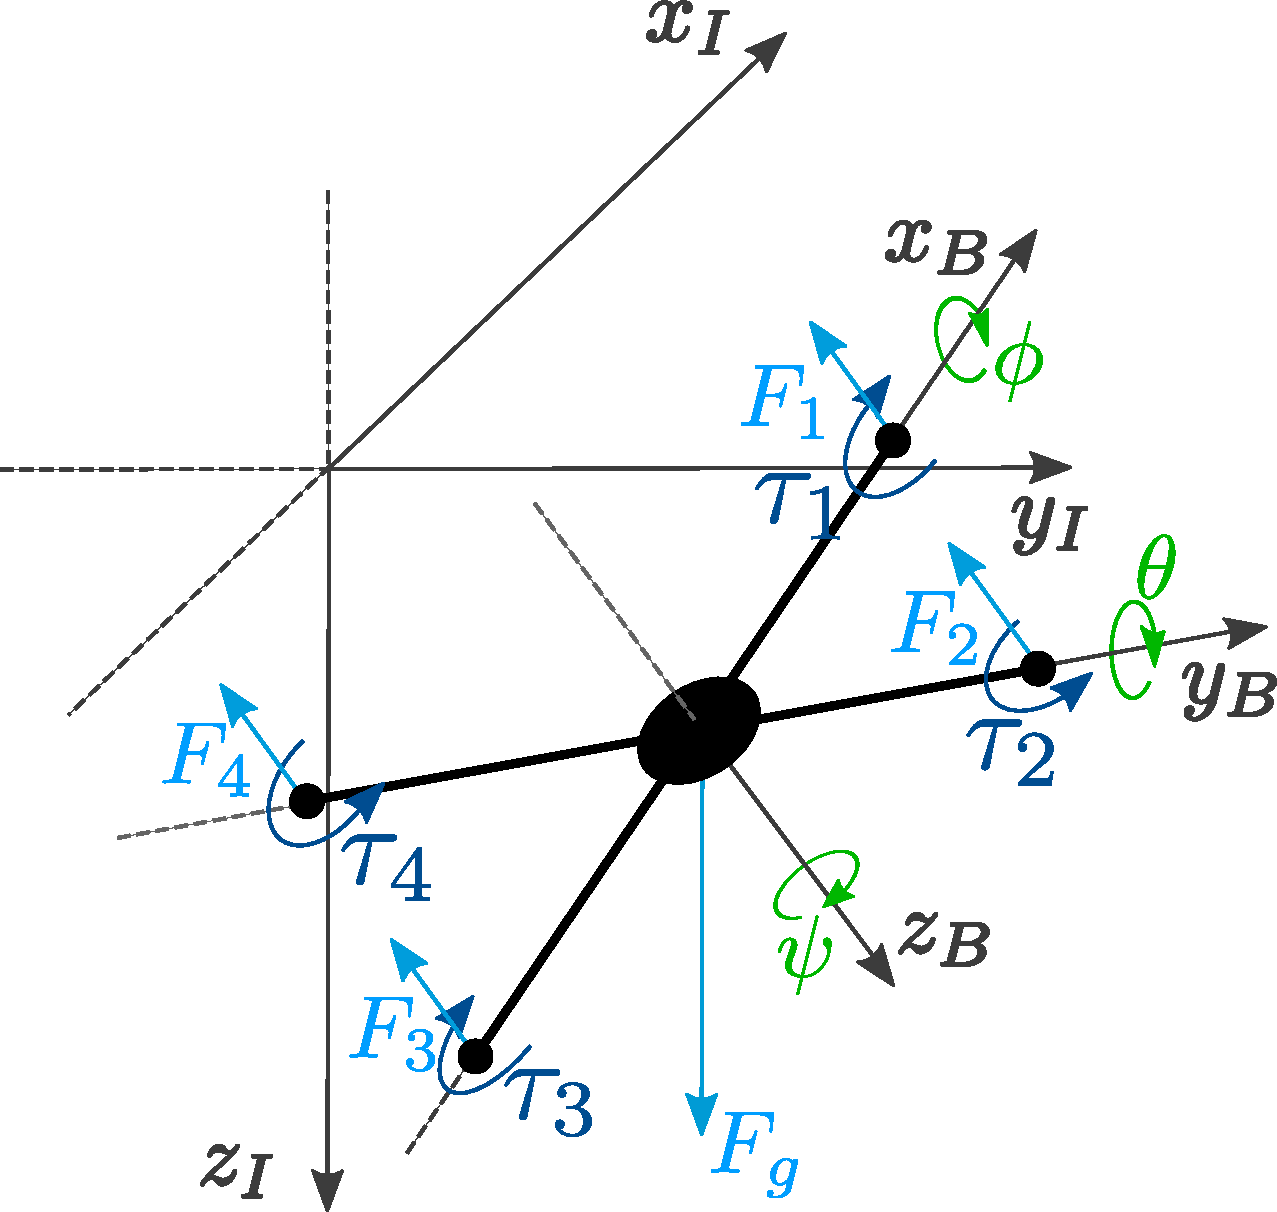
\includegraphics[scale=0.3]{figures/droneDiagram}
	\caption{Quadcopter diagram showing the forces and torques acting on the system and the positive references chosen for rotations and translations in both Inertial and Body coordinate frames.}
	\label{droneDiagram}
\end{figure}
The forces generated in the propeller are easily explained in the Body coordinate frame. In order to represent them in the Inertial frame a rotation matrix is used. It is built considering a 123 rotation sequence \cite{rotationmatrix}
 
The dynamic model of the quadcopter can be explain through three sets of equations. The first describes the motor and the propeller, the second presents the attitude response of the quadcopter and the third explains hos the translational variables of the system evolve with time.
\subsubsection{Motor and Propeller}
The four motors in the quadcopter generate the rotation required so the propeller creates the force that lifts the quadcopter. This force is called thrust force and can be modeled as proportional to the square of the motor rotational velocity. MAYBE SOURCE. The coefficient for this equation is called thrust coefficient and has been found by experiments.  
The rotation of the propellers also generates a torque on each motor due to drag between air and propeller. Drag torque is compensated in the quadcopter by having two of the motors turning in one direction and the two others in the opposite. It can also be described as proportional to the square of the velocity by terms of a drag coefficient that has also been obtained through tests.
Equation \ref{eq:thrustForce} and \ref{eq:dragTorque} show the expression for the thrust force and drag torque caused by the rotation of the propeller.
\begin{align}
	F&=k_{th}\omega^2\label{eq:thrustForce}\\
	\tau&=k_{d}\omega^2\label{eq:dragTorque}
\end{align}
\textbf{INCLUDE WHERE}\\
This equations are included in the attitude and translational models derived below.
\subsubsection{Attitude Model}
The attitude model equations are based on Newton Second Law for rotational movement and are represented in Equation \ref{eq:AngleEqVelocities1}, \ref{eq:AngleEqVelocities2} and \ref{eq:AngleEqVelocities3}. 
\begin{align}
	J_x\ddot{\phi}&=k_{th} (\omega^2_4-\omega^2_2)  L \label{eq:AngleEqVelocities1}\\
	J_y \ddot{\theta}&=k_{th} (\omega^2_1-\omega^2_3)  L \label{eq:AngleEqVelocities2} \\
	J_z\ddot{\psi}&=k_d (\omega^2_1-\omega^2_2+\omega^2_3-\omega^2_4)\label{eq:AngleEqVelocities3}
\end{align}
\textbf{INCLUDE WHERE}\\
%\begin{where}
%	\va{k_{th}}{is the thrust coefficients}{N\cdot s^2 \cdot rad^{-2}}
%	\va{k_d}{is the drag coefficients}{N \cdot m\cdot s^2 \cdot rad^{-2}}
%\end{where}
The expressions above state how the thrust force difference between motors 1 and 3 affects the roll angular acceleration, how that between motors 4 and 2 affects the pitch angle and how the yaw acceleration depends on the four motors by means of the drag torque generated on the propeller.  
\subsubsection{Translational Model}
The equations describing the response of the system along the x, y and z axes is derived from Newton's Second Law. The forces that act on the system are those from the propellers and the gravitational. These expressions are shown in Equation \ref{eq:AccelerationEqInertial1}, \ref{eq:AccelerationEqInertial2} and \ref{eq:AccelerationEqInertial3}. FIX EQUATIONS
\begin{flalign}
 	\eq{m\ddot{x}_I}{-k_{th}({\omega_1}^2+{\omega_2}^2+{\omega_3}^2+{\omega_4}^2)\sin(\theta)} \label{eq:AccelerationEqInertial1}\\
 	\eq{m\ddot{y}_I}{-k_{th}({\omega_1}^2+{\omega_2}^2+{\omega_3}^2+{\omega_4}^2)(-\sin(\phi))\cdot\cos(\theta)} \label{eq:AccelerationEqInertial2}\\
 	\eq{m\ddot{z}_I}{F_g-k_{th}({\omega_1}^2+{\omega_2}^2+{\omega_3}^2+{\omega_4}^2)\cos(\phi)\cdot\cos(\theta)}
 	\label{eq:AccelerationEqInertial3}
\end{flalign}
It is worth mentioning that, as the thrust forces always point in the negative z direction in the body coordinate frame, the accelerations in x and y directions in the inertial frame are zero as long as pitch and roll angles are 0.
\subsection{Linearization}
The linearization of the model equations has been developed following the first order Taylor approximation around an equilibrium point of the system. The chosen point is the hovering position and that implies that all variables have a value of zero, that is, the translational and attitude accelerations, velocities and positions. Choosing a zero acceleration equilibrium point along the Inertial z axis yields a equilibrium rotational speeds so that the necessary thrust is generated to compensate for the gravitational force.

The resulting equations for the attitude model after the linearization are shown in Equation \ref{eqAngleLin1}, \ref{eqAngleLin2} and \ref{eqAngleLin3}. 
\begin{flalign}
	J_x\Delta\ddot{\phi}   &= 2k_{th}L({\overline{\omega}_4} \Delta \omega_2-{\overline{\omega}_2} \Delta \omega_4)
	\label{eqAngleLin1} \\
	J_y\Delta\ddot{\theta} &= 2k_{th} L({\overline{\omega}_1} \Delta \omega_1-{\overline{\omega}_3} \Delta \omega_3) 
	\label{eqAngleLin2} \\
	J_z\Delta\ddot{\psi}   &= 2k_d({\overline{\omega}_1}\Delta \omega_1-{\overline{\omega}_2}\Delta \omega_2+{\overline{\omega}_3}\Delta \omega_3-{\overline{\omega}_4} \Delta \omega_4) \label{eqAngleLin3}
\end{flalign}
\textbf{INCLUDEWHERE}
%\begin{where}
%	\va{ \Delta\ddot{\phi}     } {is the change in roll angular acceleration from equilibrium}         { rad \cdot s^{-2} }
%	\va{ \Delta\ddot{\theta}   } {is the change in pitch angular acceleration from equilibrium}        { rad \cdot s^{-2} }
%	\va{ \Delta\ddot{\psi}     } {is the change in yaw angular acceleration from equilibrium}          { rad \cdot s^{-2} }
%	\va{ \overline{\omega}_i } {is the angular velocity of each motor in equilibrium}             { rad \cdot s^{-1} }
%	\va{ \Delta \omega_i       } {is the change in angular velocity from equilibrium of each motor} { rad \cdot s^{-1} }
%\end{where}
Similarly, the equations of the translational model are linearized. The result is shown in \ref{eq:TransLinearEquations1}, \ref{eq:TransLinearEquations2} and \ref{eq:TransLinearEquations3}. \textbf{FIX EQUATIONS}
\begin{flalign}
	m\cdot\Delta\ddot{x}_I &= -k_{th}({\overline{\omega}_1}^2+{\overline{\omega}_2}^2+{\overline{\omega}_3}^2+{\overline{\omega}_4}^2)\cos(\overline{\theta}) \Delta\theta \label{eq:TransLinearEquations1} \\
	m\cdot\Delta\ddot{y}_I &=  k_{th}({\overline{\omega}_1}^2+{\overline{\omega}_2}^2+{\overline{\omega}_3}^2+{\overline{\omega}_4}^2)\cos(\overline{\phi})\cos(\overline{\theta})\Delta\phi \label{eq:TransLinearEquations2}\\
	m\Delta\ddot{z}_I &= -2\textbf{ }k_{th}({\overline{\omega}_1}\Delta\omega_1+{\overline{\omega}_2}\Delta\omega_2+{\overline{\omega}_3}\Delta\omega_3+{\overline{\omega}_4}\Delta\omega_4)\cos(\overline{\phi})\cos(\overline{\theta})\label{eq:TransLinearEquations3}
\end{flalign} 
\textbf{INCLUDEWHERE}
%
%\begin{where}
%	\va{\Delta\ddot{x_I}  }{ is the change in linear acceleration from equilibrium in $x_I$ direction }{ m \cdot s^{-2} } \\
%	\va{\Delta\ddot{y_I}  }{ is the change in linear acceleration from equilibrium in $y_I$ direction }{ m \cdot s^{-2} } \\
%	\va{\Delta\ddot{z_I}  }{ is the change in linear acceleration from equilibrium in $z_I$ direction }{ m \cdot s^{-2} } \\
%	\va{\Delta \phi       }{ is the change in roll from equilibrium                          }{ rad            } \\
%	\va{\Delta \theta     }{ is the change in pitch from equilibrium                         }{ rad            } \\
%	\va{\Delta \psi       }{ is the change in yaw from equilibrium                           }{ rad            } \\
%	\va{\overline{\phi}   }{ is the roll in equilibrium                                      }{ rad            } \\
%	\va{\overline{\theta} }{ is the pitch in equilibrium                                     }{ rad            } \\
%	\va{\overline{\psi}   }{ is the yaw in equilibrium                                       }{ rad            }
%\end{where}                   %<--subsection
\section{Network}\label{sec:network}
The wireless network between the external sensor and the quadcopter influences the performance of the controller. This influence is considered and two effects, delay and missed packets, are examined.

%The effects on the control performance of the usage of the wireless network to get the sensor data can be divided in two. These are the delay and the packet loss. 

The theoretical modeling of these influences has been studied by several researchers with the purpose of understanding how the stability of the control system is affected when a network is used \cite{ling}, \cite{nirupam}. However, these approaches often lead to an increase in the complexity as the network effect is taken into account in the model of the system.

Stability of the system when influenced by the network is instead analyzed using the network simulator TrueTime \cite{TrueTimeNew}. It provides the ability to simulate the network model, the controller design and the system model together. This approach makes it possible to design the controllers taking into account the network effects and, thus, ensuring that stability is achieved.

The delay is modeled in the network simulation as constant for all samples. Its value is calculated by adding two time intervals. The first is the time needed for the transmission of the data, that is, the time elapsed since the data is acquired until it is available for the controller. This is a fixed delay formed by a combination of transmission and code execution times. The second is the maximum time until the controller utilizes the data. It is estimated as the sampling time minus the execution time of the control loop. This yields the maximum delay, thereby considering the worst case scenario.

The missed packets, defined as a constant probability of the controller using old data, is found experimentally by sending a large amount of packets and examining how many control loops run with old data. 
% In the experiment, it has been found that more packets are received than control loops are executed, that is, the most recent packet is always available for the controller and, therefore, the packet loss probability is zero.                 %<--subsection
\subsection{Control}
The control of the system is divided into two control systems. One handles the attitude equations and the other controls the translational variables.                  %<--subsection
\section{Attitude Controller}
The angular response of the quadcopter constitutes a coupled behavior as the three Euler angles (\si{\phi}, \si{\theta} and  \si{\psi}) are affected by the four motor velocities. This makes it harder to utilize independent controllers for each angle. A state space approach is instead considered.   

In state space, the system behavior is represented by means of the linearized model equations. These show how the output and the states of the system evolve as a function of the current states values and the input applied to the system. \autoref{xDotDiffEq} and \autoref{yDiffEq} show the idea of state space representation.
%
\begin{flalign}
	\vec{\dot{x}}(t)&=f(\vec{x}(t),\vec{u}(t))
	\label{xDotDiffEq} 
\end{flalign}
\begin{flalign}
	\vec{y}(t)&=g(\vec{x}(t),\vec{u}(t)) 
	\label{yDiffEq} 
\end{flalign}
%
The description of the system can also be expressed in matrix form, giving \autoref{xDotLinear} and \autoref{yLinear}.
%
\begin{flalign}
	\vec{\dot{x}}(t)&=\vec{A} \  \vec{x}(t) + \vec{B} \  \vec{u}(t)
	\label{xDotLinear} 
\end{flalign}
\begin{flalign}
	\vec{y}(t)&=\vec{C} \  \vec{x}(t) + \vec{D} \  \vec{u}(t)
	\label{yLinear} 
\end{flalign}
%
\begin{where}
    \va{\vec{A}}{$=\frac{\partial}{\partial \vec{x} } \ f(\vec{x_o},\vec{u_o})$ \ \ is the $6 \times 6$ state feedback matrix}{}
    \va{\vec{B}}{$=\frac{\partial}{\partial \vec{u}} \ f(\vec{x_o},\vec{u_o})$ \ \ is the $6 \times 4$  input matrix}{}
    \va{\vec{C}}{$=\frac{\partial}{\partial \vec{x}} \ g(\vec{x_o},\vec{u_o})$ \ \ is the $3 \times 6$  output matrix}{}
    \va{\vec{D}}{$=\frac{\partial}{\partial \vec{u}} \ g(\vec{x_o},\vec{u_o})$ \ \ is the $3 \times 4$  feedforward matrix}{}
\end{where}

This state space description can be seen also in the form of a block diagram like the one shown in \autoref{SSBlocks}.
%
\begin{figure}[H]
	\begin{tikzpicture}[ auto,
                       thick,                         %<--setting line style
                       node distance=1.5cm,             %<--setting default node distance
                       scale=1,                     %<--|these two scale the whole thing
                       every node/.style={scale=1}, %<  |(always change both)
                       >=triangle 45 ]                %<--sets the arrowtype
    
    \draw%-----------------------------------------------------------------------------------------
    	%Drawing Input/Output:
    	node[shape=coordinate][](input1) at (0,0){}
    	node[shape=coordinate][](output1) at (9.5,0){}
     	%Drawing the Equation Blocks:   	
      	node(A) at (4.5,-1.5) [block] {A} 
     	node(B) at (1.5,0) [block] {B}
     	node(C) at (6.5,0) [block] {C}
      	node(D) at (4.5,1.5) [block] {D}  
	    node(int) at (4.5,0) [block] {\si{\int}}  
    	%Drawing the Sumation Blocks:	    	 	
    	node(sum1) [sum, right of = B] {\si{\sum}}
    	node(sum2) [sum, right of = C] {\si{\sum}}
    	%Drawing the Feedback/Feedforward Nodes:    	
    	node[shape=coordinate][](FeedforwardNode) at (0.75,0){}
    	node[shape=coordinate][](FeedbackNode) at (5.5,0){}  	
    	     
    ;%---------------------------------------------------------------------------------------------
   
    %Joining the Blocks
  	\draw[->](input1) -- node {u}(B);
  	\draw[->](B) -- node {}(sum1);
  	\draw[->](sum1) -- node {\si{\dot x}}(int);  	
  	\draw[->](int) -- node {x}(C);
  	\draw[->](C) -- node {}(sum2);  	
  	\draw[->](sum2) -- node {y}(output1);
  	
  	\draw[->](FeedforwardNode) |- node{} (D);
  	\draw[->](D) -| node{} (sum2);

  	\draw[-] (FeedbackNode) |- (A);
  	\draw[->] (A)   -| (sum1);

    %Drawing node(s) with \textbullet
    \draw%--------------------------------------------------------------
      node at (input1)  [shift={(-0.08, -0.02 )}] {\large \textbullet}
    	% node at (output1) [shift={( 0.008, -0.02 )}] {\textbullet}
    ;%------------------------------------------------------------------
  \end{tikzpicture}
	\centering
	\caption{Block diagram of the state space representation of the system.}
	\label{SSBlocks}
\end{figure}\vspace{-18pt}
%
As the orientation of the quadcopter is to be controlled and the differential equations that describe the behavior include the angular accelerations, the state vector is chosen to be formed by the angles and the angular velocities. The input vector contains the four motor velocities and the output is constructed by the angles \si{\phi}, \si{\theta}, \si{\psi}. These vectors can be seen in \autoref{uVector}.\\
\begin{minipage}{0.32\linewidth}
	\begin{flalign}
		\vec{x}(t) = 
		\begin{bmatrix}
			\phi \\
			\theta \\ 
			\psi \\
			\dot{\phi} \\
			\dot{\theta} \\
			\dot{\psi} \\
		\end{bmatrix}	\nonumber
		\label{xVector}
	\end{flalign}  
\end{minipage}\hfill
%\hspace{0.03\linewidth}
\begin{minipage}{0.32\linewidth}
	\begin{flalign}
		\vec{y}(t) = 
		\begin{bmatrix}
			\phi \\
			\theta \\ 
			\psi \\
		\end{bmatrix}	\nonumber
		\label{yVector}
	\end{flalign}
\end{minipage}\hfill
%\hspace{0.03\linewidth}
\begin{minipage}{0.32\linewidth}
	\begin{flalign}
		\vec{u}(t)= 
		\begin{bmatrix}
			\omega_1 \\
			\omega_2 \\
			\omega_3 \\
			\omega_4 \\
		\end{bmatrix}\textsl{}
		\label{uVector}
	\end{flalign}
\end{minipage}\hfill
\\
The specific matrices for the description of the angular behavior are obtained from the linearized equations of the system (\autoref{AngleLin1}, \ref{AngleLin2}) and they are showed embedded in the state space representation in \autoref{xDotSS} and \autoref{ySS}.

\begin{flalign}   \label{xDotSS}
	\vec{\dot{x}}(t) &=
	\begin{bmatrix}
		\ 0 & 0 & 0 & 1 & 0 & 0     \ \ \ \\ 
		\ 0 & 0 & 0 & 0 & 1 & 0     \ \ \ \\ 
		\ 0 & 0 & 0 & 0 & 0 & 1     \ \ \ \\
		\ 0 & 0 & 0 & 0 & 0 & 0     \ \ \ \\ 
		\ 0 & 0 & 0 & 0 & 0 & 0     \ \ \ \\ 
		\ 0 & 0 & 0 & 0 & 0 & 0     \ \ \ 		
	\end{bmatrix}
	\vec{x}(t) +
	\begin{bmatrix}
		\ 0 & 0 & 0 & 0      \ \ \ \\ 
		\ 0 & 0 & 0 & 0      \ \ \ \\ 
		\ 0 & 0 & 0 & 0      \ \ \ \\
		\ 0 & \si{-\frac{2 \  k_{th} \  L \  \overline{\omega}_2}{J_x}} & 0 & \si{\frac{2 \  k_{th} \  L \  \overline{\omega}_4}{J_x}}      \ \ \ \\ 
		\ \si{\frac{2 \  k_{th} \  L \  \overline{\omega}_1}{J_y}} & 0 & \si{-\frac{2 \  k_{th} \  L \  \overline{\omega}_3}{J_y}} & 0      \ \ \ \\ 
		\ \frac{2 \  k_d \  {\overline{\omega}_1}}{J_z} & - \frac{2 \  k_d \  {\overline{\omega}_2}}{J_z} & \frac{2 \  k_d \  {\overline{\omega}_3}}{J_z} & - \frac{2 \  k_d \  {\overline{\omega}_4}}{J_z}      \ \ \ 		
	\end{bmatrix}
	\vec{u}(t)
\end{flalign}
\begin{flalign} \label{ySS}
	\vec{y}(t) &=	 
	\begin{bmatrix}
		\ 1 & 0 & 0 & 0 & 0 & 0     \ \ \ \\ 
		\ 0 & 1 & 0 & 0 & 0 & 0     \ \ \ \\ 
		\ 0 & 0 & 1 & 0 & 0 & 0     \ \ \ 		
	\end{bmatrix}
	\vec{x}(t)
\end{flalign}


The dynamics of the system can be analyzed by looking at the system matrix A. The eigenvalues of this matrix represent the location of the open loop poles of the system. In this case, the system shows 6 poles located in zero, which means that the system is marginally stable. In order to place those poles at a better location state feedback is used together with an integral action to be able to set a desired reference for the angles that is different from zero. 

As the output is formed by the the three angles, these are the only measured states in the system. For doing the state feedback, the angular velocities are also needed. The way of obtaining it i chosen to be a reduce order observer even though when using the vicon system, the angular velocities could be estimated with a numerical differentiation procedure. The observer is more convenient in case of using on board sensors and by using it, that possibility is kept open.

This way of approaching the control of the system is simplified by the possibility of designing the state feedback and integral controller and the observer independently. This holds due to the separation principle \cite{ssReference}.

Before designing the controller and the observer, it is advisable to check the controllability and observability of the system. For doing so, the matrices shown in \autoref{controlabilityandobservability} are used.\\
\begin{minipage}{0.45\linewidth}
\begin{flalign}
\vec{{\mathcal C}} = 
\begin{bmatrix}
\vec{B}&\vec{A}\vec{B}&\vec{A^2}\vec{B}&\vec{A^3}\vec{B}&\vec{A^4}\vec{B}&\vec{A^5}\vec{B} \\	
\end{bmatrix}\nonumber 
\end{flalign}
\end{minipage}\hfill
%\hspace{0.03\linewidth}
\begin{minipage}{0.45\linewidth}
\begin{flalign}
\vec{{\mathcal O}} = 
\begin{bmatrix}
\vec{C} \\
\vec{C}\vec{A} \\
\vec{C}\vec{A}^2 \\
\vec{C}\vec{A}^3 \\
\vec{C}\vec{A}^4 \\
\vec{C}\vec{A}^5 \\		
\end{bmatrix}					\label{controlabilityandobservability} 									
\end{flalign}
\end{minipage}\hfill

The rank of these matrices is 6, that is, the number of states. This makes the system both controllable and observable. The precise value of the matrices can be seen in \autoref{app:matricesSS}.

The block diagram showing the system overview of the attitude controller is showed in \autoref{attitudecontrollerdiagram}, in which the state feedback, the integral control and the observer can be seen.
\begin{figure}[H]
	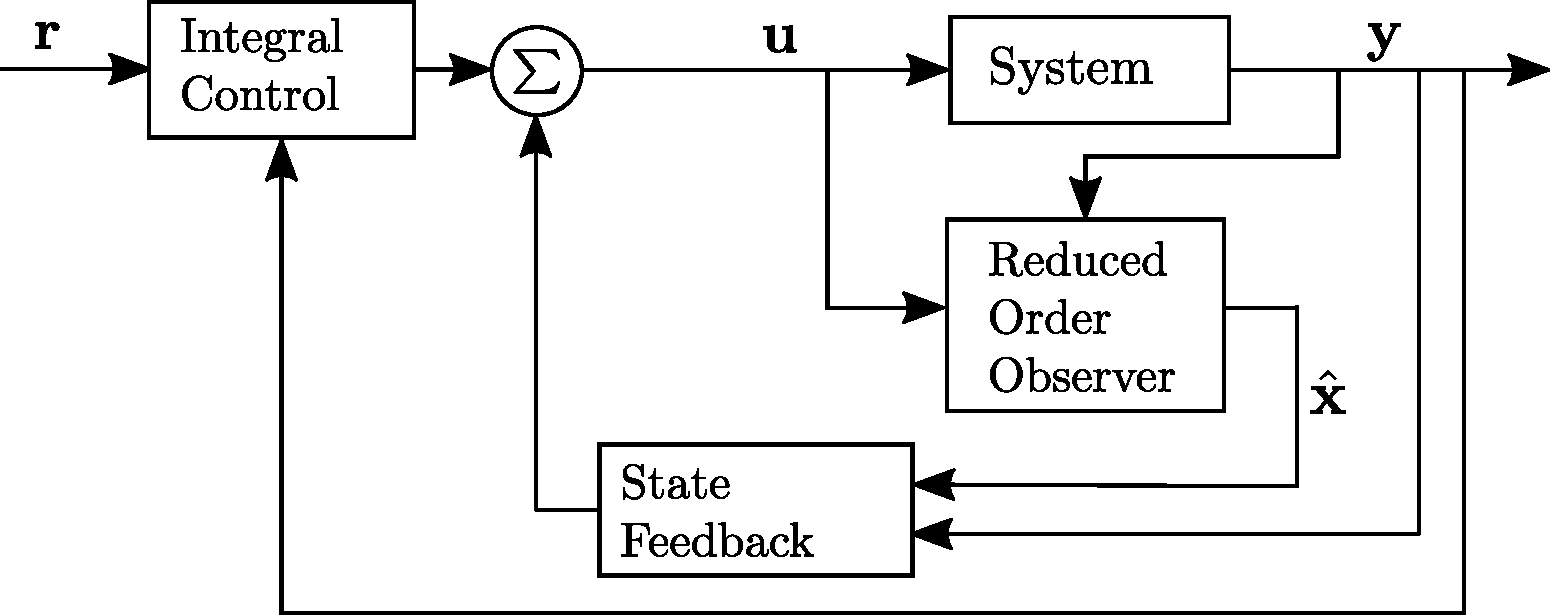
\includegraphics[scale=.5]{figures/AttitudeControlDiagram}
	\centering
	\caption{Control structure for the system, including the state feedback, the integral control and the reduced order observer.}
	\label{attitudecontrollerdiagram}
\end{figure}


      %<--subsubsection
\subsection{Translational Controller}
The translational controllers are structured as cascade loops, where the velocity and position are controlled in the inner and outer loop, respectively. The relation between the controllers is presented in \autoref{fig:cascade}.
%
\begin{figure}[H]
	\hspace{-.37cm}
	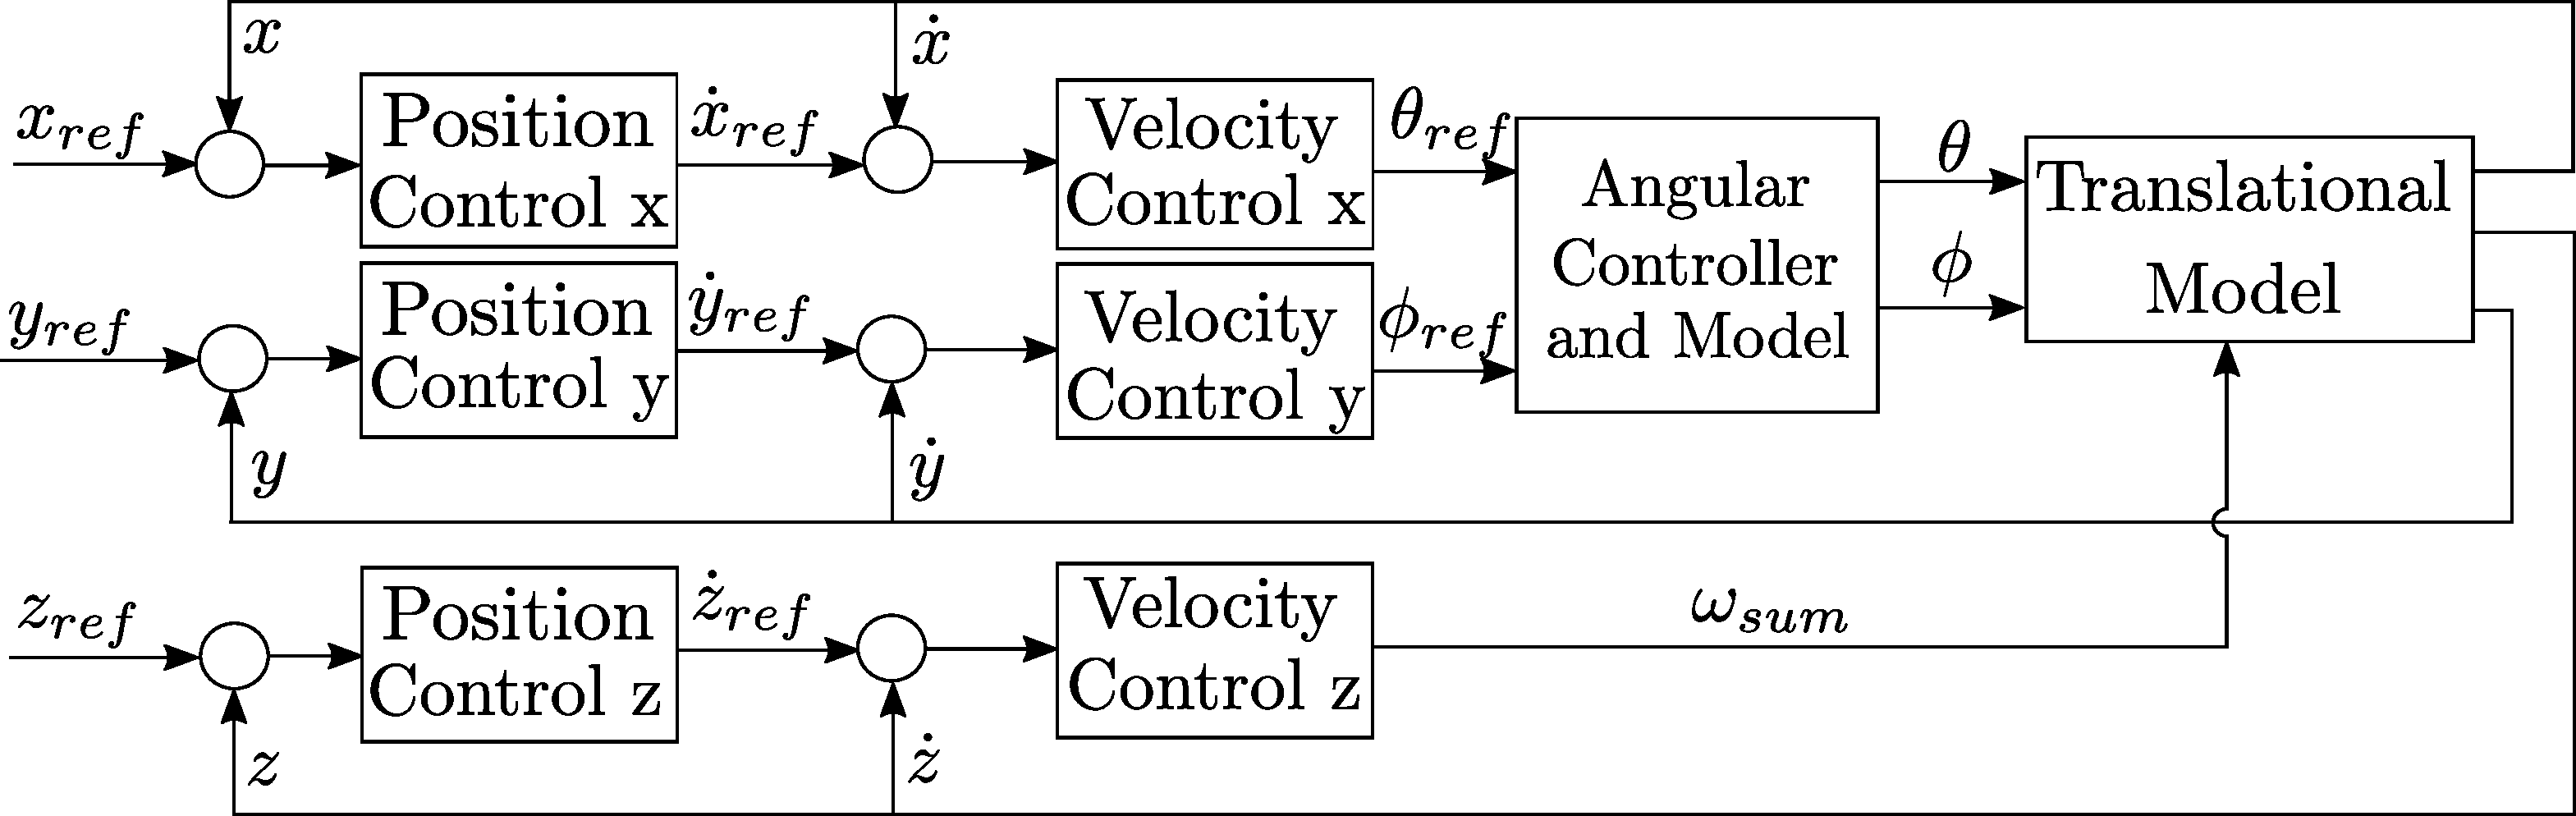
\includegraphics[width=.54\textwidth]{figures/TranslationalControlDiagram.pdf}
	\caption{Overview of translational controllers structure.}
	\label{fig:cascade}
\end{figure}

The x and y controllers share similar properties as both their outputs are angle references, $\theta_{\mathrm{ref}}$ and $\phi_{\mathrm{ref}}$, while the output of the z controller is the required sum of motor rotational speeds.\\

To design the inner controllers for the velocities $\dot{x}$ and $\dot{y}$, the model equations derived previously, see \eqref{eq:AccelerationEqInertial1} and \eqref{eq:AccelerationEqInertial2}, are Laplace transformed. These are used to create a transfer function between the angles and the velocities, yielding:
\begin{flalign}
    G_{\dot{x}}(s)&=\frac{\dot{x} (s)}{\theta (s)}=\frac{-k_{th} (\omega_1 ^2 + \omega_2 ^2 + \omega_3 ^2 + \omega_4 ^2)}{m\ s}\label{transferfunctionxdot} \\
    G_{\dot{y}}(s)&=\frac{\dot{y} (s)}{\phi (s)}=\frac{k_{th}(\omega_1 ^2 + \omega_2 ^2 + \omega_3 ^2 + \omega_4 ^2)}{m\ s}\label{transferfunctionydot} 
\end{flalign}

\noindent where $G_{\dot{x}}$ and $G_{\dot{y}}$ are the plants used to design the velocity controllers in $x_I$ and $y_I$ directions respectively.

Since the plants are the same but with different signs, the controller design is carried out for $\dot{x}$ and applied to $\dot{y}$ afterwards with negative sign.

A proportional controller is chosen as the plant already has an integrator, which eliminates steady state tracking error and the effect of output disturbances. The gain is designed such that the system has a bandwidth that is three times lower than the attitude control loop to ensure that its dynamics do not affect the designed controller. %\cite{bandwidthReference}.

The outer loop is again designed to have three times less bandwidth than the inner velocity loop. Then, the plant of the outer loop is only an integrator that transforms velocity to position. As for the inner loop, the controller of the outer loop is a proportional controller. \\

To be able to design the inner loop for the z translational controller, the model equation derived previously, see \eqref{eq:AccelerationEqInertial3}, is Laplace transformed and written on the form of a transfer function, see
%
\begin{align}
G_{\dot{z}}=\frac{\dot{z}}{\omega_{sum}} &= \frac{ \frac{1}{4}\ (-2 k_{th})\ \overline{\omega}_{sum} }{ m\ s }\label{eq:linearTransferFunctionZ}
\end{align}

\noindent where $\dot{z}$ is the velocity in the $z_I$ direction, $\omega_{sum}$ is the sum of the rotational speeds of the motors and $\overline{\omega}_{sum}$ is the sum of the rotational speeds in equilibrium.

Due to an integrator and a negative gain the system's root locus will move into the right half plane as the gain increases. A proportional controller with negative gain ensures the system to be stable. 

As there is not any inner control loop, input disturbances may occur such that a steady state error appears, which is not eliminated by the integrator in the plant. To remove this potential error an integrator is added to the controller. 

The plant for the z position controller is just an integrator and a proportional controller is utilized. This is as well designed so that the bandwidth frequency is three times lower than the inner one.
 %<--subsubsection

%-----RESULTS-----------------------------------------------------------
\section{Results}
Simulation vs. reality. \\
%Design a setup that allows a nice measurement of reality - yet to be done\\
Comment on the results and how that correlates with reality, without discussing possible issues or improvements.
Model parameters: \fxnote{bring table with values}
Controllers:
Attitude controller:
Translational controller:

The inner loop proportional controller of the x and y translational cascade controllers are as follows:
\begin{align}
C_{\dot{x_I}}(s)= -0.19\\
C_{\dot{y_I}}(s)= 0.19
\end{align}

The outer loop  proportional controller of the x and y translational cascade are as follows:
\begin{align}
C_{\dot{x_O}}(s)&= 0.55\\
C_{\dot{y_O}}(s)&= 0.55
\end{align}

%
%-----DISCUSSION--------------------------------------------------------
\chapter{Discussion}
%
%-----CONCLUSION--------------------------------------------------------
\section{Conclusion}
In this project, the behavior of a quadcopter has been modeled by first principles of physics. A control system has been designed in order to hover and move to a desired position.
The control system has been split into an attitude and a translational controller. The first one has been designed using a state space approach, including state feedback with integral control and a reduced order observer. The translational control system has been designed with a classical control approach and result in three cascade loops, including proportional and PI controllers. 
As the quadcopter uses an external motion tracking system to determine its position and orientation, an analysis of the issues that can arise when having a networked distributed system has been done in order to ensure the control system remains stable. The performance of the controllers shown in the results demonstrates the efficiency of the control strategy reveal in the paper.


%---------------------------------------------------------
%
%FUTURE WORK---------------------------------------------
\section{Future Work}\label{sec:futurework}
The control system has been designed using an external motion tracking system as sensor for attitude and position. This system limits the operation area of the quadcopter. A future step could be to implement alternative sensors located on the quadcopter to further investigate the capabilities of the control structure and to enable outdoor flight.
 %able to fly outside the improve the result while keeping the same control structure, an inertial measurement unit could be installed on the quadcopter.  
%
%-----ACKNOWLEDGMENTS---------------------------------------------------
\section{Acknowledgments}
%Henrik Schiøler , associated professor at Aalborg University \\
%Christoffer Sloth, associated professor at Aalborg University
\fxnote{commented out until final version is to be handed in}
%
%-----BIBLIOGRAPHY------------------------------------------------------
\printbibliography

\end{document}